
%%%%%%%%%%%%%%%%%%%%%%%%%%%%%%%%%%%%%%%%%%%%%%%%%%%%%%%%%%%%%%%%%%%%%%%%%%%%%%%%%%%%%%%%%%%%%%%%%%%%%%%%%%%%%%%%%%%%%%%%%%%%%%%%%%%%%%%%%%%%%%%%%%%%%
%%%%%%%%%%%%%%%%%%%%%%%%%%%%%%%%%%%%%%%%%%%%%%%%%%%%%%%%%%%%%%%%%%%%%%%%%%%%%%%%%%%%%%%%%%%%%%%%%%%%%%%%%%%%%%%%%%%%%%%%%%%%%%%%%%%%%%%%%%%%%%%%%%%%%
%%%%%%%%%%%%%%%%%%%%%%%%%%%%%%%%%%%%%%%%%%%%%%%%%% FIRST LECTURE: EVENTS %%%%%%%%%%%%%%%%%%%%%%%%%%%%%%%%%%%%%%%%%%%%%%%%%%%%%%%%%%%%%%%%%%%%%%%%%%%%%
%%%%%%%%%%%%%%%%%%%%%%%%%%%%%%%%%%%%%%%%%%%%%%%%%%%%%%%%%%%%%%%%%%%%%%%%%%%%%%%%%%%%%%%%%%%%%%%%%%%%%%%%%%%%%%%%%%%%%%%%%%%%%%%%%%%%%%%%%%%%%%%%%%%%%
%%%%%%%%%%%%%%%%%%%%%%%%%%%%%%%%%%%%%%%%%%%%%%%%%%%%%%%%%%%%%%%%%%%%%%%%%%%%%%%%%%%%%%%%%%%%%%%%%%%%%%%%%%%%%%%%%%%%%%%%%%%%%%%%%%%%%%%%%%%%%%%%%%%%%

\section{Events and Sample Space}
Motivated by the Introduction~\ref{s:intro} we first introduce the notion of events. We then see that events can be modelled using set theory, after introducing the sample space

\subsection{Definition of an event}
In light of the subjective perspective on Probability Theory we will refer to the person who is evaluating the probabilities of events using "you". Following \cite{definetti}  we can define events as 
\begin{definition}
    \label{d:event}
    An event is an unambiguous statement which can be either true or false and about which you are uncertain.
\end{definition}
Informally, unambiguous statement means that a possible bet or insurance based upon it can be decided without question. 
Examples of events are: " The next ChatGPT sentence will be incorrect" or " Napoleon was born on March" ( to decide this last statement, I should open Wikipedia). 
Events will be usually denoted by capital letters, $A$, $B, \ldots$, and the impossible event will be usually denoted by $\emptyset$. 




\subsection{Operations and relations between events}
\label{ss:operations}

From two events $E$ and $F$ it is possible to consider new events using the operations "or" "and", and "not", namely, to consider $"E \textrm{ and }   F"$, $ "E \textrm{ or } F"$ and "$\textrm{ not } F$". To make a simple example let E= "I will obtain my Ph.D" and F=" Tomorrow it will rain". Then   

\begin{itemize}

	\item "E and F"= " Tomorrow it will rain and I will obtain my Ph.D ".
	\item "E or G"= "Tomorrow either it will rain or I will take my Ph.D ".
	\item "not E"= " I will not take my Ph.D".

\end{itemize}

Given two events E or F we say that $E$ implies $F$ and we write (for reasons that will become clear in the following) $E \subset F$ if, $F$ is true whenever $E$ is. If $G $ = "Tomorrow it will rain heavily", then $G \subset F$. Note that in general 
	\begin{itemize}
		\item $"E$ and $F$" $\subset  E$. \\
		\item $ F \subset "E  \text{ or}  F"$. 
	\end{itemize}


\subsection{Elementary Events and Sample Space}

There are no inherent restrictions on the events one can define and on which you could try to assign a probability. When doing a probabilistic study, you might wish to restrict your attention and consider only particular events. For example, if we are interested in the result of a coin toss we are interested in the event E="The result of the coin toss is tails" but not on the event "The result of the coin toss is tails and tomorrow it will rain in Rome".\\

\begin{example}
	You are paid by a shop owner to perform a statistical analysis of the number and the kind of customers visiting his shop. For time and economic constraints, you have to choose what kind of events you are interested in. One possibility is to consider only the number of customers, so that events will be of the form "More than 10 customers will visit the shop", " 3 customers will visit the shop"... \\
	In the case the shop owner is also interested in the gender of the customers, you might wish to consider events that take into account the number of customers and their genders, such as "More than 3 male customers and less than 10 female customers will visit the shop", "2 male and 1 female will visit the shop". 
\end{example}

From now on we assume that we have always set beforehand the events that we want to consider.  We assume that given two events $E$ and $F$ that we want to consider, then any of the events that can be built from them is an event that we want to consider
\begin{definition}[Measurable events]
	\label{d:measurable}
	The set of \emph{events we want to consider} $\mathfrak F$ is a set of events that is closed under intersection: If $E, F  \in \mathfrak F$ then also $E\cap F \in \mathfrak F$ (if we want to consider $E$ and $F$ we also want to consider "$E$ and $F$"). 
\end{definition}

\begin{example}[Coin Toss]
	\label{ex:cointoss}
	If we toss a coin and we are interested only in the face shown by it, then the events that h we want to consider are those that can be written in terms of theface shown by the coin: consists on the events we can write using the   interested is 
	\begin{equation}
		\label{}
			\begin{split}
				\mathfrak F & = \left\{ \emptyset,\text{ "The coin gave heads"}, \text{"The coin gave tails"}, \right.\\
					& \qquad \left.\text{"The coin gave either H or T" }\right\}.
			\end{split}
	\end{equation}

\end{example}

Once the events we want to consider are fixed and collected in $\mathfrak F$ it is possible to define a particular kind of events, the \emph{elementary events} thanks to which we can model events using set theory. Informally, elementary events are the smallest among the events we want to consider, and can be regarded as the outcome of the "experiment" we are observing. It is indeed possible to define a notion of smallness using using the relation "implies" which we have denoted by $\subset$ is Section~\ref{ss:operations}. An event $E$ is "smaller" than $F$ if $E \subset F$, and the elementary events are simply the smallest events we want to consider.     
\begin{definition}[Elementary Events]
	\label{d:elementary}
	We say that an event $ E \in \mathfrak  F$  is elementary if for any other event $F$ that we want to consider, then $F$ does not imply $E$. That is, $E$ is elementary if for any $F \in \mathfrak F$ with $F \subset E$, then $ F = E$.  
\end{definition}
\begin{ExerciseList}
	\Exercise Show that two different elementary events are mutually disjoint, that is, that if $E$ and $F$ are elementary and $E \neq F$, then "$E$ and $F$" = $\emptyset$. 
	\Answer In light of the assumptions made in Definition~\ref{d:measurable}, $"E \text{ and } F " \in \mathfrak F$. Since $" E \textrm{ and } F \subset E$, if the event $"E \text{ and } F" $ is possible, it contradicts Definition~\ref{d:elementary}
\end{ExerciseList}

The notion of elementary events is fundamental since it allows to see all the previously introduced quantities as already encoded using set theory, with which everyone is familiar 
\begin{definition}[Sample Space]
	\label{d:sample_space}
	Given $\mathfrak F$, the sample space $\Omega$ is the set of elementary events. 
\end{definition}
Elements of the sample space, that is, elementary events, are usually denoted with $\omega$.  The sample space can be regarded as the set of possible oucomes of the system you are looking at with the degree fo precision that you want to impose. Some examples are in order. 

\begin{example}[Sample Space of a Coin Toss ]
	If $\mathfrak F$ is the one defined in \eqref{ex:cointoss}, then the elementary events are $\omega_1 =$ " The result is heads" and $\omega_2$ = " The result is tails", and the sample space is $\Omega = \{\omega_1, \omega_2\}$. Note that we can use a different notation and set $ 0 = \omega_1$ and $ 1 =\omega_2$. However, $0$ and $1$ are must not be mistakes for numbers (numbers are usually associated to unit of measures) . They are symbols indicating elementary events 

\end{example}

\begin{example}[a die is rolled]
		\label{ex:die_sample}
		If a die is rolled, we migh wish to look at events of the form "The result of the die is an even number". Elementary events, the ones that cannot be decomposed just by looking at the die, are 1= "The result is 1" , ..., 6= "The result is 6". The sample space is therefore $\Omega =\{1,2,3,4,5,6\}$ and, again,the elements 1,...,6 must not be mistaken for numbers, since are elementary events and, for instance, 1 + 3 doesn't make sense. 

\end{example}

\begin{example}[A chess match]
If you observe a chess match the events you want to consider are those that involve the game alone, such as " The game will end before 10 moves are taken" or "Black wins", while the elementary events are the possible single games. Therefore, the sample space is the set of all possible games. A full description of a game is usually given in terms of the so called algebraic notation. An example of a match is given by ( a Fisher vs. Kasparov match)  is given by \\
1.d4Nf6 2.c4e6 3.Nc3Bb4 4.Nf3c5 5.e3Nc6 6.Bd3Bxc3+ 7.bxc3d6 8.e4e5 9.d5Ne7 10.Nh4h6 11.f4Ng6 12.Nxg6fxg6 13.fxe5dxe5 14.Be3b6 15.O-OO-O 16.a4a5 17.Rb1Bd7 18.Rb2Rb8 19.Rbf2Qe7 20.Bc2g5 21.Bd2Qe8 22.Be1Qg6 23.Qd3Nh5 24.Rxf8+Rxf8 25.Rxf8+Kxf8 26.Bd1Nf4 27.Qc2Bxa40–1\\
	The algebraic notation can be seen as a way to encode elementary events and the sample space. In Exercise~\ref{e:game} and \ref{exercise:game_2} examples of sample spaces defined by simple games are given    

\end{example}





\subsection{Exercises}

\begin{ExerciseList}
	\Exercise
       From the 2019-2020 course " Mathematics and Statistics" given by  professors 
       Khovanskaya, Bubilin, Shurov, Filimonov and Sonin at HSE.\\ 
       A six faced die is rolled. Find the elementary events that imply the event
    
      \Question "The result is 6"
      \Question "The result is a number less or equal 2"
      \Question "The result is an even number"
      \Question "The result is a number strictly greater than 4"
      \Question "The result is seven"  
    
% 	\Answer 
%	
%	\Question It is already an elementary event 
%	\Question "The result is a number less or equal than 2"= "The result is 1" or "The result is 2". 
%	\Question "The result is a number strictly greater than 4" = "The result is 5" or "The result is 6 ". 
%	\Question The event is the impossible event, also denoted by $\emptyset $. 
%
	\Exercise  A coin is tossed twice. We are interested in the face which the coin shows when it lands: heads or tails. The set of elementary events is $\{ HH, HT,TH,TT\}$, where the event HH corresponds to "the first toss gave heads, the second heads", the event HT corresponds... Write the elementary events that imply the events
   
         \Question "We obtained two heads".
         \Question "The first toss gave heads".
         \Question "We obtained 1 tails "
         \Question "At least one toss gave tails"
        
%    	\Answer 
%
%	\Question $ HH$.
%	\Question $ TH, TT$.
%	\Question $TH, HT$.
%	\Question $HT, TH, TT$.
	
    \Exercise A coin is tossed 4 times. We are interested in the face that it shows when it lands: heads or tails. How many elementary events are there? which elementary events are contained in the events 
    
    
      \Question The first result was heads
      \Question The second result was tails
      \Question The first result was heads and the second tails 
      \Question All the 4 tosses gave the same result
    
%	\Answer  The elementary events are HHHH, HHHT,HHTH,....,TTTT. There are $2^4=16$ of them.
%
%	\Question HHHH, HHHT,....,HTTT 
%	\Question HTHH,HTHT,HTTH,...,TTTT
%	\Question HTHH, HTHT,HTTH,HTTT
%	\Question  HHHH, TTTT
%
	\Exercise (\cite{Ross} Chapter 2 Exercise 1)
	\label{exercise:marbles}
  A box contains 3 marbles: 1 red, 1 green, 1 blue. Consider the experiment that consists in taking 1 marble from the box and then replacing it in the box and then drawing a second marble. Describe the sample space.\\
 	
%	\Answer The sample space can be thought as the set of the outcomes of the experiment. In this case the possible outcomes are "The first marble is red and the second marble is red", "The first marble is red and the second is green",... A more efficient way to write an outcome is to write an array with two entries, i.e, (r,g), where the first entry represents the colour of the firs marble, and the second entry represents the colour of the second marble. That is, we write the elementary event "The first marble is red and the second is blue" by (r,b). The sample space becomes 
% \bel{ex1}{\Omega=\{(r,r), (r,g),(r,b),(g,r), (g,g),(g,b),(b,r),(b,g),(b,b)\}}
 
 	\Exercise
 Repeat Exercise 1 when the second marble is drawn without replacing the first marble.\\
 	
%	\Answer The outcomes (r,r), (g,g) and (b,b) are no longer possible. The sample space is 
% \bel{ex2}{\Omega=\{(r,g),(r,b),(g,r),(g,b),(b,r),(b,g)\}}
     
	\Exercise
You toss a coin 3 times. Describe the elementary events.\\
%	\Answer $\Omega=\{(H,H,H), (H,H,T),....,(T,T,T)\},$ where the event (H,T,H) is "The result of the first toss was head, the result of the second...". 

\end{ExerciseList}


\subsection{ Events as Subsets of the Sample Space}
	\label{ss:subset}
%The minimality of the elementary events implies that the following property holds. If $\omega \in \Omega$ and $E \in \mathfrak F$, then either $\omega \subset E$ or $\omega \cap E  =\emptyset$. 
\begin{definition}[Elementary events favourable to an event]
	We say that an elementary event $\omega \in \Omega$ is in favour of $E \in \mathfrak F$ if $\omega$ implies $E$. 
\end{definition}
The minimality of the elementary events implies that for each $E \in \mathfrak F$ and $\omega \in \Omega$ either $\omega$ is in favour of $E$ or they are mutually exclusive (that is, $ \text{"$\omega$ and $F$"} = \emptyset$). We can associate to each event the subset of $\Omega$ whose elements are the elementary events that imply $E$: 
\begin{equation}
	\label{e:abstract_to_concrete}
	\begin{array}{ccc}
		\Phi: \mathfrak F & \mapsto & \{ \text{subset of $\Omega$}\} = \{A\,, A \subset \Omega\}\\
		E & \to & \{ \omega \in \Omega \, ,  \omega \subset E\} 
	\end{array}
\end{equation}
\begin{example}[Dice]
		\label{ex:die_subset}
	We have seen in Example~\ref{ex:die_sample} that the sample space of a dice that is rolled can be identified with $\Omega = \{1,2,3,4,5,6\}$. The elementary events that are favourable to $E $ = "The result is an odd number" are $1,3,5$. Therefore we identify $E$ with the subset of $\Omega$ given by $\{1,3,5\}$. 	
\end{example}

From now on we will consider $\mathfrak F$ as a set of subsets of $\Omega$. The fundamental fact of the identification of events with subsets of $\Omega$ given by $\Phi$ is that the operations "or", "and" and "not" correspond to the operations of $\cup$, $\cap$ and $ ()^c$, respectively, and that $E$ implies $F$ if and only if $E$ is a subset of $F$. For instance, in the die example, if $E$ = "The result is an odd number" and $F$ = "The result is greater than 2", then  "E and F" = " The result is an odd number greater than 2". The first two events are identified with the subsets of $\Omega$ given by $\{1,3,5\}$ and $\{3,4,5,6\}$, while "E and F" is identified with $\{3,5\}$, which is exactly the intersection of the two sets. \\

We can now model events using set theory and we can depict them using Venn's diagrams, as shown in picture \ref{f:Venn} 
\begin{figure}[h]
	\includegraphics[width = 10cm]{Venn.jpg}
	\caption{ Venn's diagram\label{f:Venn}}
\end{figure}
	 

Points in the sample space are events on their own and it might be helpful to consider them as events in a larger and refined sample space $\Omega$. This will be done rigorously is Section~\ref{s:sys}

\begin{example}[Two dice rolled]
	\label{ex:sum_restriction}
	Two dice have been rolled and suppose that we can only look ate the sum of tehir results. The sample sspace is therefore $\Omega = \{2,3,4,\ldots, 12\}$. If one is allowed to look at each die, then the sample space is $\Omega' = \{11,12,\ldots, 66\}$, and the elementary events in $\Omega$ are not anymore elementary ( apart from 2 and 12) in $\Omega'$. Figure~\ref{f:sum_dice} repressents this situation, which will be made rigorous in Example~\ref{ex:su}

\begin{figure}[h]
\includegraphics[width = 5cm]{Sum_of_Dice.png}
\label{f:square}
\end{figure}

\end{example}

	Another reason for which we would like to consider the points of $\Omega$ as events of in a lager sample space $\Omega'$ is that the latter can cointain many different sample spaces, as the next example shows. This fact will be again detailed in Section~\ref{s:sys} and, in particular, in Subsection~\ref{ss:cartesian}. 
	\begin{example}
		\label{ex:two_coin_sample}
		The sample space of a coin toss can be identified with $\Omega = \{H, T\}$, and if we toss another coint the sample space is again the same. If we consider a large $\Omega'$, depicted in Figure~\ref{f:square}, that contains also the two coin tosses, see Figure~\ref{f:1toss} and \ref{f:2toss}, then we can consider also the sample space of the two coins $\tilde \Omega = \{HH,HT,TH,TT\}$, see Figure~\ref{f:twotosses}.   

\begin{figure}[h]
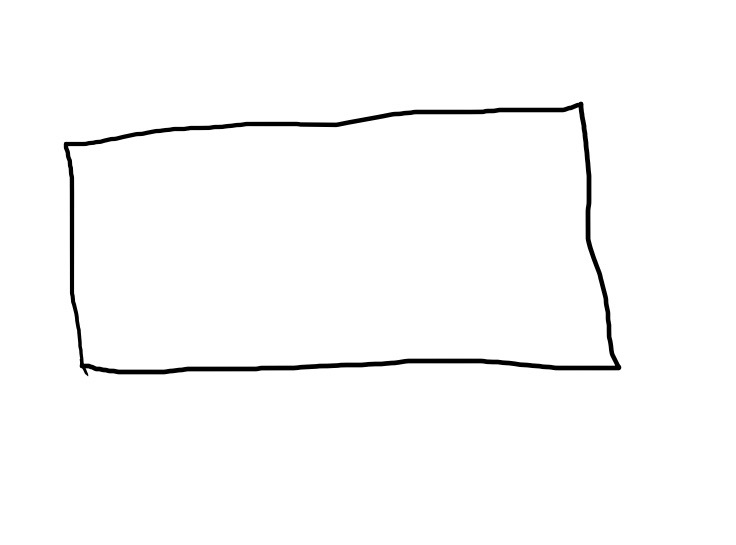
\includegraphics[width = 5cm]{Square.jpg}
\label{f:square}
\end{figure}


\begin{figure}[h]
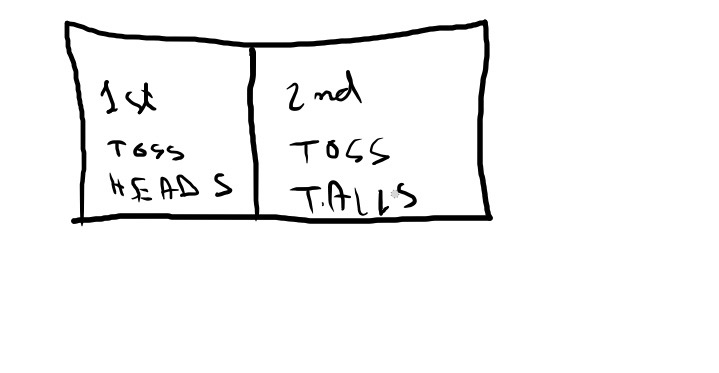
\includegraphics[width = 5cm]{firsttoss.jpg}
\label{f:1toss}
\end{figure}

		\begin{figure}[h]
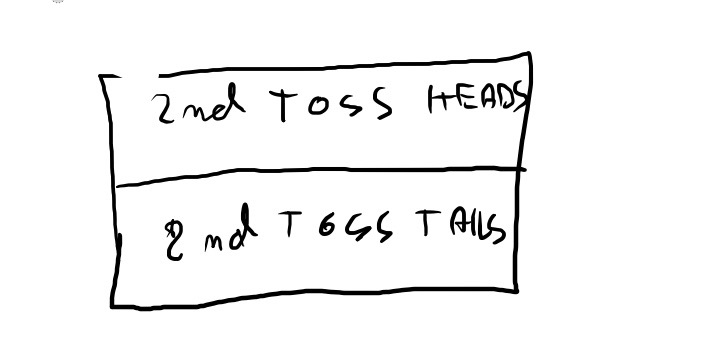
\includegraphics[width = 5cm]{secondtoss.jpg}
\label{f2toss}
\end{figure}

\begin{figure}[h]
\includegraphics[width = 5cm]{twotosses.jpg}
\label{f:twotosses}
\end{figure}
		Finally, we can look refine the sample space with other events, see Figure~\ref{f:tossandrain}. 

\begin{figure}[h]
\includegraphics[width = 5cm]{twotossesandrain.jpg}
	\caption{ We can refine the sample space with other events \label{f:tossandrain}}
\end{figure}

	\end{example}
 

\begin{ExerciseList}
	\Exercise (\cite{Feller}, Chapter 1.8) Let $\Omega$ be a sample space and $A,B, C$ be three arbitrary events. Find the expressions for the events that of $A,B,C$:
        \Question Only $A$ occurs.
	\Question  Both $A$ and $B$, but not $C$ occur. 
	\Question  All three events occur. 
	\Question  At least one occurs.
	\Question  At least two occur. 
	\Question  One and no more occurs.
	\Question  Two and no more occur 
	\Question  None occurs. 
	\Question  Not more than two occur.
	
%	\Answer
%
%	\Question	$A\setminus (B\cup C)=A\cap B^c \cap C^c$.
%	\Question	$ (A\cap B)\setminus C = A\cap B \cap C^c$.
%	\Question	$ A\cap B \cap C$.
%	\Question	$ A\cup B \cup C$.
%	\Question	\label{ex:set1} At least two occur if occur one bertween $A\cap B$, $A\cap C$ or $B\cap C$. Thus $ (A \cap B)\cup (A\cap C) \cup ( B \cap C)$. 
%        \Question        It has to happen one between $A$ $B$ and $C$, that is, it has to happen $A\cup B \cup C$, but it does not have to happen two of them, that is, it cannot happen the event described in \ref{ex:set1}: 
%	\Question	  $ (A \cap B)\cup (A\cap C) \cup ( B \cap C)$. Thus the event is $A\cup B \cup C \setminus ((A \cap B)\cup (A\cap C) \cup ( B \cap C))$.
%	\Question	$ \left((A \cap B) \cup (A \cap C) \cup (B \cap C) \right)\setminus A \cap B \cap C $ which is the same as  $ \left((A \cap B) \cup (A \cap C) \cup (B \cap C) \right) \cap (A^c \cup B^c \cup  C^c) $ .
%	\Question	$(A\cup B \cup C)^c= A^c\cap B^c \cap C^c$. 
%	\Question	This event happens when the event all three events occur does not happen. Thus the event is $(A \cap B \cap C)^c =A^c \cup B^c \cup C^c. $
%
\end{ExerciseList}

\subsection{Examples}

\begin{example}[A Coin Toss]
If in a coin toss we are interested only in the face the coin shows, as we always are when we speak about coin tosses, then the only two non-tricial events we want to consider are  0=" The result is tails" and 1 = " The result is heads", see also Example~\ref{ex:cointoss} and \ref{ex:die_subset}. Therefore 
	\begin{equation}
		\Omega_1=\{0,1\},
	\end{equation}
	and we will ofter refer to $1$ as to a success. The set of events that we want to consider can be represented by 
	\begin{equation}
		\mathfrak F = \{\emptyset, \{0\}, \{1\},\{0,1\}\}.
	\end{equation}
\end{example}

\begin{example}[two, three and $n$ coin tosses]
	\label{ex:n_coin}
The sample space of two coin tosses can be encoded by $\Omega_2=\{00,01,10,11\}= \{x_1x_2\,,\, x_i\in\{0,1\} i=1,2\}$, where, for example, 
If we toss twice a coin and we are only interested in the faces they show, then we are interested in events of the form " The first coin shows heads" or "The second coin shows tails". The smallest events we can make by intersecting this kind of events are of the form 01="The first toss gave tails and the second tails". Therefore the sample space is constituted by the set 
	\bel{}{
		\Omega_2 = \{00,01,10,11\} = \{x_1x_2, x_i \in \{0,1\}, \text{ for $i = 1, 2$}  \} 
	} 
	of two digit string where every digit represents the outcome of the respective coin. 
	Similarly, for 3 coin tosses 
	\bel{}{\Omega_3=\{000,001,010,011,100,101,110,111\}=\{x_1x_2x_3\,,\,x_i\in\{0,1\} i=1,2,3\},} 
	 and, in the general case of $n$ coin tosses, the sample space is the space of strings of $n$ digit with values in $\{0,1\}$, namely 
	\begin{equation}
		\label{e:ntoss}
		\Omega_n = \{x_1x_2\ldots x_n\, , x_i \in \{0,1\} , i = 1,\ldots, n\}. 
	\end{equation}
	Events that we will often use when introducing the Binomial distribution, see Example~\ref{????} are the events $E_k$= "There has been exactly $k$ successes", for $k \in \mathbb N$, $k < n$. For instance, if $n = 3$ and $k = 1$, is $E_1=\{001,010,100\}=\{x_1x_2x_3\,,\,x_1+x_2+x_3=1\}$. The particular encoding given by \eqref{e:ntoss} allows us to write in simple terms the condition imposed by $E_k$:
	\begin{equation}
	\label{e:ntoss_ksuccesses}
		E_k = \{ x_1\ldots x_n \in \Omega_n \,, x_1 + \ldots + x_n = k \}.
	\end{equation}
\end{example}

\begin{example}[Finite but Undetermined Amount of Coin Tosses]
If we are observing a finite amount of coin tosses, but we do not know how many of them there will be, we can define the set of possible outcomes, that is, the sample space, via the following encoding  
\begin{equation}
    \label{e:finite_coin}
	\begin{split}
	\Omega= & \bigcup_{i=1}^\infty \Omega_i = \{0,1,00,01,10,11,000, \ldots \},\\
		& = \left\{ x_1\ldots x_n , n \in \mathbb N, x_i \in \{0,1\}, \text{ for $i = 1,\ldots n$}\right\}
	\end{split}
\end{equation}
	where $\Omega_i$ has been defined \ref{e:ntoss}. 

\end{example}

\begin{example}[Infinite Coin Tosses]
	\label{ex:infinite_coin}
If we are observing an infinite amount of coin tosses, then the sample space is the set of strings whose digits denote the result of the corresponding coin. 
	\begin{equation}
		\label{e:infinite_coin}
 \Omega=\{x_1...x_n...\, ,\, x_i\in\{0,1\}\}.
	\end{equation}
	 Possible events that we would like to take into account are of the form "The first toss gave $a_1$, the second $a_2$,..., the nth $a_n$", where $n \in \mathbb N$ and $a_{i} \in \{0,1\}$ for $i = 1, \ldots, n$. This event correspods to the subset of $\Omega$ consisting on strings whose first $n$ elements are $a_i$, for $i = 1,\ldots, n$
		\begin{equation}
			\label{e:infinite_coin_set}
			A_{a_1,\ldots, a_n} = \{x_1\ldots x_n\ldots \in \Omega\,\, x_1 = a_1, \ldots, x_n = a_n \}.
		\end{equation}
\end{example}

\begin{example}[ Random Number Between 0 and 1]
	\label{ex:unif}
	By typing on R the command runif, the computer gives us a number $X$ between 0 and 1. 
\begin{knitrout}
\definecolor{shadecolor}{rgb}{0.969, 0.969, 0.969}\color{fgcolor}\begin{kframe}
\begin{alltt}
\hlkwd{runif}\hldef{(}\hlnum{1}\hldef{)}
\end{alltt}
\begin{verbatim}
## [1] 0.7328875
\end{verbatim}
\end{kframe}
\end{knitrout}
	Some events in which we are usually interested are " $X < 1/2$ ", " $X \in [1/4, 1/ 2) $". By intesecating the above events we can see, at least intuitively, that the smallest events one can make are $X = x$. The sample space is therefore composed by the events "$ X = a $" for each $a \in [0,1]$, and, by denoting $a$ the event $ X = a$, 
	\bel{e:unif_1}{
		\Omega = \{\text{" $X = a$"}, a \in [0,1]\} = [0,1].
	} 
The set of events we want to consider $\mathfrak F$ contains the events of the form $ X \in [a,b]$, where $0 \leq a <  b \leq 1 $, if we are using the notation in the centre of \eqref{e:unif_1}, and $[a,b]$ if we are using the other notation for $\Omega$.    
\end{example}

	Example~\ref{ex:infinite_coin} and ~\ref{ex:unif} constitute are different from the previous ones. In both cases the spaces are too big to be written as a list of elements, that is, in the form $\Omega = \{ \omega_1 , \omega_2, \ldots \}$. In jargon, $\Omega$ is not discrete. The difficulty is that now the specification of $\mathfrak F$ becomes important since, for good  mathematical reasons, it is in general not possible to consider each $A \subset \Omega$.

%\begin{example}[undetermined, possibly infinite amount of coin tosses ]
%$\Omega=\bigcup_{i=1}^\infty\Omega_i \cup \tilde{\Omega}$
%\end{example}
%As we will see, in exercises what is usually given is the sample space, and next section shows that every event can be obtained from the sample space.  
%Generally, in the statement of the exercises is given an experiment with its elementary events (or outcomes of the experiment). One task you should be able to do is to recognize them and encode them in a smart way. \\
%









\subsection{Exercises}


\begin{ExerciseList}
	\Exercise
	\label{exercise:game_2}
    (\cite{Ross} Chapter 2 Exercise 2) In an experiment, die is rolled continually until a 6 appears, at which point the experiment stops. What is the sample space of this experiment? Let $E_n$ denote the event " The experiment is completed before n rolls". Write it as a subset of the sample space. Describe $\left(\bigcup_{i=1}^\infty E_i\right)^c$.

%\Answer The sample space is the space of outputs of the experiment. We encode the event "The first roll gave 4, the second 2, the third 6 and then stops" in the string 426. That is, we encode the output of the experiment in strings of digits 1,2...,5,6,  where the digit correspond to the result of the die, and the position of the digit corresponds to when has the digit appeared. The string must stop at after the first 6, since the game stops when the die gives 6. \\We have to keep in mind that we can observe events in which we never stop rolling the die, which correspond to infinite strings of 1,2...5, for example 1212121.... or  121233...34453236.... 
%\bel{}{\Omega=\{ 6, 16, 26, 36, 46, 56,116,...\}\cup\{x_1x_2....x_n...\,: x_{i}\in\{1,2,3,4,5\} \}=E\cup G.}
%The set $E$ is the event that the game stops in a finite number of rolls. The set $G$ is the event that the game goes on without ending. For any reasonable probability, the event G has probability 0, and it is usually neglected. 
%The events $E_i$ can be written as subsets of the state space in the following way: $E_1=\{6\}$, $E_2=\{6,16,26...,56\}$, $E_3=E_2 \cup \{116,126,...,556\}$,... (In a more compact form $E_i=\{x_1...x_n6\,:\, x_i\in\{1,...,5\}\, n\leq i\}$).

%The event $$\bigcup_{i=1}^\infty E_n= E_0\cup E_1\cup E_2,....= "E_0\,\, or E_1 \,\,or ....E_n \,\,\,or ..."$$
%is, by definition of "or", the event that $E_n$ happens for at least one $n$. That is, is the event "The game ends before $n$ rolls at least one $n$ "="The game ends after $n$ rolls for some $n$", which coincides with $E$.
%The set event $E^c$ corresponds to $G$. 

\Exercise (\cite{Ross} Chapter 2 Exercise 3)
Two dice are thrown. Let $E$ be the event that the sum of the dice is odd, and $F$ the event that at least one of the two dice lands in $1$ and let $G$ be the event that the sum is 5. Describe the events $E\cap F $, $E\cup F$, $F\cap G$, $E\cap F^c=E\setminus F$ and $E \cap F\cap G$

%\Answer
% $$E=\{(1,2),(1,4),(1,6),(2,1),(2,3),(2,5),(3,2)...(6,5)\}$$
% $$F=\{(1,1),(1,2),(1,3),(1,4),(1,5),(1,6),(2,1)...(6,1)\} $$
% $$
% G=\{(1,4),(2,3),(3,2),(4,1)\}
% $$
% $$
% E\cup F=\{(1,1),(1,2),(1,3),(1,4),(1,5),(1,6),
% (2,1),(2,3),(2,5),(3,1),(3,2),(3,4)..(6,5)\}
% $$
% $$E\cap F=\{(1,2),(1,4),(1,6),(2,1),(4,1),(6,1)\}$$
% $$
% F\cap G=\{(1,4),(4,1)\}
% $$
% $$
% E\cap F\cap G=F\cap G=\{(1,4),(4,1)\}
% $$
% $$
%E\cap F^c=\{((2,3),(2,5),(3,2),(3,4),(3,6),(4,3),...(6,5)\}$$
%
\Exercise 
\label{e:game}(\cite{Ross} Chapter 2 Exercise 4)
Anton, Barbara  and Carlo take turns flipping a coin. The first one to get head wins. The sample space to this experiment can be defined as $\Omega=\{1,01,001,0001,...\}\cup\{00000...\}$.
\Question Interpret the sample space.
\Question In terms of the sample space, write the following events: A="Anton wins", B="Barbara wins" and $(A\cap B)^c$.

%\Answer \Question 1="First toss is heads"(So that Anton wins)  01="The first toss is tails, the second heads "(So that Barbara wins)... The event 00000...="Head never arises, the game never stops". 
%
%	\Question As it is easy to seen, Anton wins whenever the digit 1 appears in the 1st, 4th, 7th.. position. This means that 
%$$
%A=\{1,0001,0000001,...\}.
%$$
%In the same way, the event that Barbara wins corresponds is 
%$$B=\{01,00001,00000001,...\}$$
%where the digit appears in the after $3\times k+1$ zeros, for some $k\in\mathbb{N}$.
% $(A\cup B)^c=\Omega\setminus(A\cup B)=\{001,000001,...\}\cup\{0000...\}$.
%The event $(A\cup B)^c$ is the event "Carlo wins or the game doesn't end"  
%
\end{ExerciseList}
